\chapter{Patch antenna design}

\section{Design Procedure of Patch Antenna}

(All formulas from \autoref{eq:width} to \autoref{eq:y0} is taken from \citep{bog} the formulas from \autoref{eq:Z0} to \autoref{eq:x2} is from \citep{web})

Before a patch antenna can be designed, it is important to find out on which substrate it should be designed for. This gives some parameter for the height, $h$ and the relative dielectric constant, $\epsilon_r$. Equally important is to determine the frequency for which the patch antenna should work for, $f$. When these parameters have been determined the actual design can begin. The width is found using \autoref{eq:width}.

\begin{equation}\label{eq:width}
w = \frac{c}{2f} \cdot \sqrt{\frac{2}{ \epsilon_{r}+1}}
\end{equation}
\begin{where}
\va{$w$}{is the width of the patch antenna}{m}
\va{$c$}{is the speed of light}{$\frac{m}{s}$}
\va{$f$}{is the chosen frequency}{Hz}
\va{$\epsilon_r$}{is the relative dielectric constant}{1}
\end{where}

Before the length of the patch can be found the effective dielectric constant needs to be found using \autoref{eq:Eeff}. 

\begin{equation}\label{eq:Eeff}
\epsilon_{eff} = \frac{\epsilon_{r}+1}{2} +\frac{\epsilon_{r}-1}{2}\cdot\left(1+\frac{12h}{w}\right)^{-\frac{1}{2}}
\end{equation}
\begin{where}
\va{$\epsilon_{eff}$}{is the effective dielectric constant}{1}
\va{$h$}{is the height of the substrate}{m}
\end{where}

The total length of the patch include both the length of the patch itself but also the electromagnetic extension from the edges. So to find the length of the patch itself can thus be found using \autoref{eq:Leff}.

\begin{equation}\label{eq:Leff}
L_{eff} = L-2\cdot\Delta L
\end{equation}
\begin{where}
\va{$L_{eff}$}{is the length of the patch antenna}{m}
\va{$L$}{is the total radiating length of the patch antenna}{m}
\va{$\Delta L$}{is the extension of the length from the patch antenna}{m}
\end{where}

The extension of the length is found using \autoref{eq:DeltaL}

\begin{equation}\label{eq:DeltaL}
\Delta L = h\cdot0.412 \frac{(\epsilon_{eff}+0.3)\left(\frac{w}{h}+0.264\right)}{(\epsilon_{eff}-0.258)\left(\frac{w}{h}+0.8\right)}\cdot 10^{-3}
\end{equation}

The total radiating length is found using \autoref{eq:L}
\begin{equation}\label{eq:L}
L = \frac{c}{2\cdot f\cdot\sqrt{\epsilon_{eff}}}
\end{equation}

Now that the physical dimensions of the patch has been found a feed needs to be made. In this case a strip line feed is chosen. Since the equipment including cables and connectors are 50 ohm this will be the desired match. The impedance in the patch varies from edge through the patch and to the other edge with 0 ohm in the center and $\approx 240$ ohm at the edge. The desired feed point is then found using \autoref{eq:y0}. 

\begin{equation}\label{eq:y0}
y_0 = \frac{\arccos\left(\sqrt{\frac{R_{in}(y=0)}{R_{in}(y=y_0)}}\right)\cdot L}{\pi}
\end{equation}
\begin{where}
\va{$y_0$}{is the insert feed point}{m}
\end{where}

The gap between the feed line and the patch has through simulations been shown to decrease performance, meaning the smaller the gap the better the performance. The gap is chosen to 0.25 mm as a minimum production width. 

The feed line needs to matched to 50 ohm also, this is done by adjusting the width of the feed line. The width can be found using \autoref{eq:Z0} to \autoref{eq:x2}.

\begin{equation}\label{eq:Z0}
Z_0=\frac{\eta_0}{2\pi\sqrt{2}\sqrt{\epsilon_r+1}}\cdot \ln\left(1+4\cdot \left(\frac{h}{w_{eff}}\right)\cdot (X_1+X_2)\right)
\end{equation}
\begin{where}
\va{$Z_0$}{is the desired impedance}{$\Omega$}
\va{$\eta_0$}{is the free space impedance = 120 $\pi$}{$\Omega$}
\va{$w_{eff}$}{can be found in \autoref{eq:weff}}{m}
\va{$X_1$}{can be found in \autoref{eq:x1}}{1}
\va{$X_2$}{can be found in \autoref{eq:x2}}{1}
\end{where}


\begin{equation}\label{eq:weff}
w_{eff} = w_{f}+\left(\frac{t}{\pi} \right) \cdot \ln \left(\frac{4\text{e}}{\sqrt{\left(\frac{t}{h}\right)^2+\left(\frac{t}{w_{f}\pi+1.1t\pi}\right)^2}}\right)\cdot \frac{\epsilon_r+1}{2\cdot \epsilon_r}
\end{equation}
\begin{where}
\va{$w_{f}$}{is the width of the feed line}{m}
\va{$t$}{is the thickness of the feed line}{m}
\va{e}{is Eulars number $\approx 2.718$}{1}
\end{where}

\begin{equation}\label{eq:x1}
X_1 = 4\cdot \left(\frac{14 \epsilon_r +8}{11 \epsilon_r}\right)\cdot \left(\frac{h}{w_{eff}}\right)
\end{equation}

\begin{equation}\label{eq:x2}
X_2 = \sqrt{X_1^2+\left(\frac{\epsilon_r+1}{2\cdot \epsilon_r}\right)\cdot\pi^2}
\end{equation}


\section{Dimensions of Patch Antennas}

The patch antennas have been designed for a FR4 board with a height of 1.6 mm and a copper thickness of 35 $\micro$m.

\begin{table}[H]
\centering
\begin{tabular}{l|lll}
                & \textbf{868MHz} & \textbf{2.4GHz} & \textbf{Unit} \\\hline
\textbf{Width}  & 105.7           & 38.2            & mm            \\
\textbf{Length} & 82.7            & 29.6            & mm            \\
\textbf{Feedpoint}  & 29.5            & 10.9            & mm            \\
\textbf{Feed Width}  & 3.06            & 3.06            & mm           
\end{tabular}
\caption{Calculated parameters}
\label{tab:parameters}
\end{table}


\begin{figure}[H]
\captionsetup{belowskip=0em}
\begin{subfigure}[b]{0.48\textwidth}
\missingfigure{868MHz}
\caption{Designed patch for 868 MHz}
\label{fig:868Patch}
\end{subfigure}
\begin{subfigure}[b]{0.48\textwidth}
\missingfigure{2400MHz}
\caption{Designed patch for 2.4 GHz}
\label{fig:2.4Patch}
\end{subfigure}
\captionsetup{belowskip=-1.5em}
\caption{The manufactored patch antennas}
\end{figure}


\section{Measured Performance}

The antennas have been tested in Satimo Starlab see \autoref{fig:satimo}. 
The radiation pattern can be seen on ??, and gain for vertical and horizontal polarization can be seen in ??. 


\begin{figure}[H]
\centering
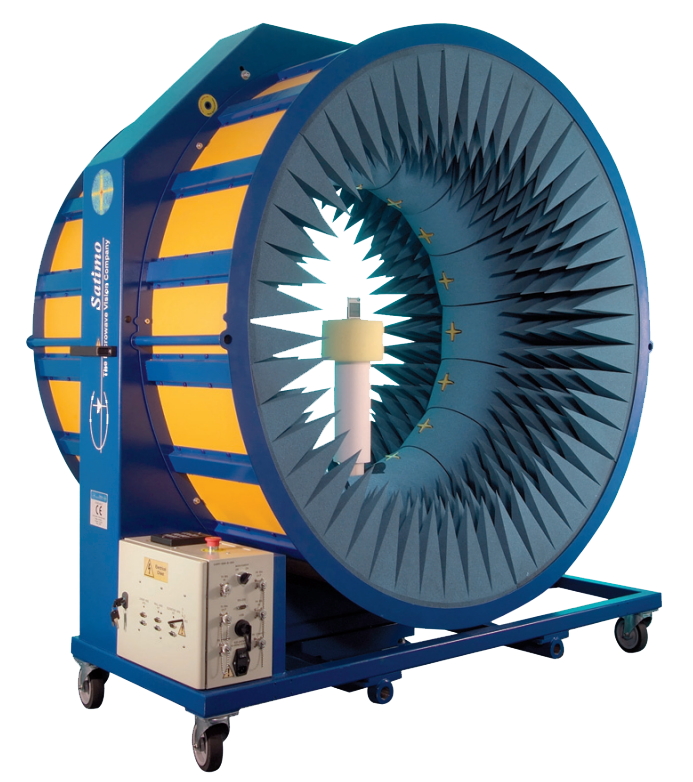
\includegraphics[width=0.3\textwidth]{figure/starlab.png}
\caption{Satimo starlab}
\label{fig:satimo}
\end{figure}
